\chapter{Evaluation}
\label{chap:evaluation}

In this chapter, we experimentally evaluate our implementation of the framework discussed in \crefrange{chap:visualizing-static-input-graphs}{chap:visualizing-dynamic-input-graphs}. The following research questions drive our evaluation:

\begin{enumerate}
	\item Which quantitative measures best capture the quality of the maps generated by our algorithm in terms of
	\begin{enumerate}
	\item accuracy?
	\item our understanding of locally fat regions?
	\end{enumerate}
	\item What is the quality of the maps generated by our algorithm according to these quality metrics?
	\begin{enumerate}
	\item How does this quality change based on the size and other properties of the input graph?
	\item How does this quality change over time as dynamic updates are incorporated?
	\end{enumerate}
\end{enumerate}

First, we discuss a variety of possible quality metrics from literature and how they can be applied to our framework in \cref{sect:quality-metrics}.
We pick two metrics that best capture the quality of the generated maps according to research question 1.
In \cref{sect:test-case-generation}, we present the algorithm we use to generate randomized test instances on which we perform our experimental evaluation.
In \crefrange{sect:implementation-and-experiment-setup}{sect:experimental-evaluation}, we conduct the actual experimental evaluation on a large number of test instances and see how the maps generated by our algorithm perform, thereby answering research question 2.
Eventually, in \cref{sect:exemplary-maps}, we showcase a range of maps produced by our framework.

\section{Quality Metrics}
\label{sect:quality-metrics}

We start by looking at common quality metrics of cartograms, which are closely related to the problem we are trying to solve in this thesis as previously discussed in \cref{sect:related-work}, and discussing how they translate to the visualizations our framework creates.
We then discuss different ideas to formalize and quantify the previously mentioned notion of local fatness of the regions.



\paragraph{Quality Metrics of Cartograms}

Three well-established quantifiable measures are commonly used to assess a cartograms's quality \cite{alam2015quantitative} \cite{nusrat2018evaluating}:

\begin{itemize}
\item \textbf{Statistical accuracy:}
The statistical accuracy of a cartogram describes how closely the areas of the modified geographic regions match the variable of interest.
Recall that the normalized cartographic error of a region $v$ is defined as $\frac{\abs{A^\prime(v)-w(v)}}{max(A^\prime(v),w(v))}$ where $A^\prime(v)$ is its normalized actual area and $w(v)$ is its desired area.
The maximum and average normalized cartographic error over all regions in the cartogram are commonly used to quantify its statistical accuracy.
We borrow this quality metric from cartograms as we have already used it previously to define $\varepsilon$-proportional maps.

\item \textbf{Topological accuracy:}
The topological accuracy describes how well the original adjacencies between the geographic regions are preserved in the cartogram.
Considering our framework computes a polygonal contact representation of the filtered cluster graph, those and only those regions whose corresponding vertices are adjacent in the cluster graph are adjacent in the contact representation.
In terms of topological accuracy, we therefore produce perfect drawings.

\item \textbf{Geographic accuracy:}
The geographic accuracy of a cartogram describes to what degree the shapes and positions of the distorted regions resemble their original counterpart on the real geographic map.
In our case, however, there is no real geographic map that our visualization is based upon:
The maps we generate are entirely artificial and there is no geographic reference map.

However, the motivation behind geographic accuracy as a quality metric still makes sense in our setting.
Geographic accuracy captures the preservation of the viewer's mental map between the real geographic map and the distorted map in the cartogram.
And this applies to our framework as well, albeit only once we start incorporating dynamic updates into the artificial map.
Our dynamic pipeline naturally preserves the viewer's mental map by only allowing small, incremental changes to be incorporated and redrawing the artificial map using a force-directed algorithm.
This makes it easy for the viewer to track how the map changes between versions of the underlying cluster graph at different points in time.
\end{itemize}



\paragraph{Polygon Complexity}

Brinkhoff \etal{} \cite{brinkhoff1995measuring} propose a method to quantify the complexity of polygons.
They measure the complexity of polygons as a combination of three properties: the frequency of the vibration of its boundary, the amplitude of said vibration, and the deviation from its convex hull.
Given a polygon $P$, they count the number of corners where the polygon's internal angle is more than $180^\circ$, called \emph{notches}, and define the fraction of those corners as
%
\begin{equation*}
\text{notches}_{\lbrack0,1\rbrack}(P) \coloneqq
\begin{cases}
\frac{\text{notches}(P)}{n - 3} & \text{if $n$ > 3}\\
0 & \text{otherwise}
\end{cases}
\in \lbrack0,1\rbrack
,
\end{equation*}
%
where $n$ is the total number of corners in $P$ and $\text{notches}(P)$ the number of corners that are notches.
They use this fraction to define the frequency of the vibration as
%
\begin{equation*}
\text{freq}(P) \coloneqq 1
+ 16 \cdot (\text{notches}_{\lbrack0,1\rbrack}(P) - 0.5)^4
- 8 \cdot (\text{notches}_{\lbrack0,1\rbrack}(P) - 0.5)^2
\in \lbrack0,1\rbrack
\end{equation*}
%
and its amplitude as
\begin{equation*}
\text{ampl}(P) \coloneqq
\frac{\text{circumference}(P) - \text{circumference}(\text{hull}(P))}{\text{circumference}(P)}
\in \lbrack0,1\rbrack
,
\end{equation*}
%
where $\text{circumference}(P)$ is the the length of $P$'s boundary and $\text{hull}(P)$ is the convex hull of $P$'s corners in the form of another polygon.
These equations were chose such that the frequency $\text{freq}(P)$ of the vibration of a polygon reaches its maximum when half of the polygon's corners are notches, and the amplitude $\text{ampl}(P)$ of the vibration is close to 1 when the area of the polygon is very small in relation to the area of it's convex hull.
Intuitively, for convex polygons $P$, both the frequency $\text{freq}(P)$ and the amplitude $\text{ampl}(P)$ of the vibration of its boundary is zero.

To measure the convexity of a polygon, Brinkhoff \etal{} use the fraction of the area of the polygon's convex hull that the polygon itself covers:
%
\begin{equation*}
\text{conv}(P) \coloneqq
\frac{\text{area}(\text{hull}(P)) - \text{area}(P)}{\text{area}(\text{hull}(P))}
\in \lbrack0,1\rbrack
\end{equation*}

According to their observations, a relative increase of the boundary in combination with a high-frequency vibration of the boundary has the most significant impact on the intuitive perception a polygon's complexity \cite{brinkhoff1995measuring}.
They therefore combine these three properties as
%
\begin{equation}
\text{compl}(P) \coloneqq
0.8 \cdot \text{ampl}(P) \cdot \text{freq}(P) + 0.2 \cdot \text{conv}(P)
\in \lbrack0,1\rbrack
\end{equation}
%
to measure the overall complexity of a polygon.

We adopt this definition of polygon complexity as a quality metric for the maps generated by our framework, but only with a slight change because as is, $\text{compl}(\cdot)$ assigns a perfect score of $0$ to all convex polygons.
This means that, for example, there is no distinction between a square region and a long, drawn-out rectangular region, even though the square regions matches our understanding of local fatness much better.
Instead of calculating the fraction of area a polygon $P$ doesn't cover within its convex hull, we therefore compute the fraction of area it doesn't cover in its smallest enclosing circle.
To keep $\text{conv}(\cdot)$ in unit interval, we actually compare $P$'s area to the maximal area of a regular $n$-gon in said smallest enclosing circle:
%
\begin{equation*}
\text{compl}^\prime(P) \coloneqq
1 - \frac{\text{area}(P)}{\text{area}(\text{smallestEnclosingCircle}(P)) \cdot \sin\left(\frac{360^\circ}{n}\right) \cdot \frac{n}{2\pi}}
\in \lbrack0,1\rbrack
\end{equation*}

In our tests, this measure has shown to align with our intuitive understanding of local fatness nicely.



\paragraph{Entropy}

Chen and Sundaram \cite{chen2005estimating} studied the complexity of 2-dimensional shapes in the field of computer vision.
The shapes they dealt with are given in the form of a point cloud.
For each point, they compute the Euclidean distance to the point cloud's centroid.
They also implement a heuristic to predict the contour of the shape at each point and use it to compute a local angle for each of the points.
The distances and local angles are then plotted into a histogram with flexible bin size and are used to compute the entropy of the distribution of distances and local angles.

In our use case, we don't even have to implement the heuristic to guess the shape's contour.
We know that the points form a closed curve that is in fact a polygon.
However, by connecting the points in this predetermined manner, we possibly get drastically different edge lengths.
The points on these edges that aren't corners of the polygon have no impact on the computed entropies at all.
This problem becomes obvious when we consider two straight-line segments of the same length, one that is a single side of our polygon, and one which is the union of multiple sides of our polygon with corners (with internal angle $180^\circ$) in between:
The one with additional corners has a much greater impact on the computed entropies, even though both look the same to an observer.

We can try to remedy by subdividing the polygon's sides first, creating roughly uniform side lengths.
However, in doing so, we create lots of corners at which the polygon has an internal angle of $180^\circ$, quickly dominating and distorting the entropy of internal angles.

In our tests, neither of two entropy-based measures, with or without our adjustments, captured our intuitive understanding of local fatness satisfactorily.
We therefore conduct our experimental evaluation in \cref{sect:experimental-evaluation} using just cartographic error and our modified version of polygonal complexity from Brinkhoff \etal{} \cite{brinkhoff1995measuring} discussed above.
For both measures, we will look at both the maximum and average value over all regions in the map.

\clearpage
\section{Test Case Generation}
\label{sect:test-case-generation}

We implement a randomized test case generation in two phases.
First, we generate a filtered cluster graph $G^\mathcal{C}$.
We accompany this cluster graph with a planar straight-line drawing $\Gamma^\mathcal{C}$ thereof so that such a drawing doesn't need to be calculated in retrospect as previously discussed in \cref{sect:transformation-to-dual}.
Second, we generate a sequence of dynamic operations to be applied to said cluster graph.

\paragraph{Filtered Cluster Graph Generation}

Our test case generation can be configured using the following five parameters:
%
\begin{itemize}
\item \textbf{Number of clusters:} The number of clusters $n \in \mathbb{N}, n \geq 3$ determines how many vertices the generated cluster graph $G^\mathcal{C}$ has.
\item \textbf{Bounding box:} The axis-aligned bounding box $\mathcal{A} = \lbrack x_\text{min}, x_\text{max} \rbrack \times \lbrack y_\text{min}, y_\text{max} \rbrack$ determines the area in which the cluster graph's vertices can be placed.
\item \textbf{Weight distribution:} The cluster weight distribution is given as a probability mass function $\pmf \colon \mathbb{N}_+ \to \mathbb{R}_+$ and determines how the cluster weights are distributed.
\item \textbf{Nesting ratio:} The nesting ratio $\alpha \in \lbrack 0, 1 \rbrack$ determines what fraction of the $n$ vertices are nested into other triangular faces.
\item \textbf{Nesting bias:} The nesting bias $\beta \in \lbrack 0, 1 )$ determines to what degree nesting vertices into already-nested triangular faces is preferred over nesting vertices into top-level triangles.
\end{itemize}

The idea behind generating filtered cluster graphs $G^\mathcal{C}$ is as follows:
We start by placing a number of vertices randomly within the bounding box $\mathcal{A}$ and computing a triangulation of these vertices.
We then place the remaining vertices into existing triangles based on the nesting ratio $\alpha$ and bias $\beta$, inserting additional edges to those triangles' endpoints in the process.
The algorithm is illustrated in pseudocode in \cref{alg:randomized-filtered-cluster-graph-generation} on the next page.

Obviously, the generated graph is plane and internally triangulated.
Considering a point set's triangulation covers the same area as the set's convex hull, no vertex of the generated graph can appear on its outer face more than once and the graph is therefore also biconnected.

Due to the independent sampling of vertex positions in \cref{alg:randomized-filtered-cluster-graph-generation}, vertices often clump together, especially for larger test instances.
This isn't an ideal starting position for the transformation as previously discussed in \cref{sect:transformation-to-dual} because the polygonal dual contains at least twice the number of vertices, therefore clumping even more and severely restricting the involved vertices' movement.
To address this issue, we apply a force-directed \quoted{shake} to the generated straight-line drawing $\Gamma^\mathcal{C}$ of the cluster graph while preserving its edge crossing and combinatorial properties.

We do this by defining attractive forces between pairs of adjacent vertices and strong repulsive forces between non-adjacent vertices and between edges and non-incident vertices based on their distances, and again applying the rules of ImPrEd \cite{simonetto2011impred} to prevent the introduction of edge crossings.
The repulsive forces are the same as the ones defined in \cref{sect:drawing-the-dual}, although we use a higher scaling constant of $1000$ here to really prevent the vertices from clumping together.
For the attractive force between adjacent vertices, we apply the force $F_\text{att}(u,v) \coloneqq \log(d(u,v) / 100)$ to both endpoints of an edge, directed towards each other.
Here, the value of $100$ represents our ideal edge length.
This force is based on a logarithmic springs as suggested by Eades \cite{eades84heuristic}.

\vfill

\begin{algorithm}[H]
	\caption{Randomized Filtered Cluster Graph Generation}
	\label{alg:randomized-filtered-cluster-graph-generation}
	\SetArgSty{textrm}
	\vspace{5pt}
	\KwData{bounding box $\mathcal A$, weight probability mass function $\pmf(\cdot)$, count $n$, nesting ratio $\alpha$, nesting bias $\beta$}
	\KwResult{planar straight-line drawing $\Gamma^\mathcal{C}$ of a filtered cluster graph $G^\mathcal{C}$ on $n$ vertices}
	\vspace{5pt}
	create empty straight-line drawing $\Gamma^\mathcal{C}$\;
	$k \gets \min(\floor{\alpha \cdot n}, n - 3)$ \tcp{number of nested vertices}
	\BlankLine
	\tcp{sample $n - k$ pairwise distinct points $p_i \in \mathcal{A}$}
	\ForEach{index $i \in \lbrack 0, n-k ) \cap \mathbb{N}$}{
		sample random point $p_i$ within $\mathcal{A}$ (uniformly)\;
		sample random weight $w_i$ (according to $\pmf(\cdot)$)\;
		add vertex $i$ with weight $w_i$ at position $p_i$ to $\Gamma^\mathcal{C}$\;
	}
	\BlankLine
	\tcp{create edges according to Delaunay triangulation of points}
	\ForEach{triangle $\triangle_j = (u,v,w) \in$ Delaunay triangulation of points $(p_i)_i$}{
		\ForEach{$(a,b) \in \{ (u,v), (v,w), (w,u) \}$}{
			insert edge between $a$ and $b$ in $\Gamma^\mathcal{C}$ unless edge already exists\;
		}
		register triangular face $\triangle_j$ with $\text{depth}(\triangle_i) = 1$\;
	}
	\BlankLine
	\tcp{nest remaining $k$ vertices into existing triangles}
	\ForEach{index $i \in \lbrack n - k, k ) \cap \mathbb{N}$}{
		sample random triangle $\triangle_i$ (weighted by $(1 - \beta)^{-\text{depth}(\cdot)}$)\;
		sample random point $p_i$ within $\triangle_i$ (uniformly)\;
		sample random weight $w_i$ (according to $\pmf(\cdot)$)\;
		add vertex $i$ with weight $w_i$ at position $p_i$ to $\Gamma^\mathcal{C}$\;
		add edges between $i$ and all of $\triangle_i$'s endpoints to $\Gamma^\mathcal{C}$\;
		unregister triangular face $\triangle_i$\;
		register the three new triangular faces with depth $1 + \text{depth}(\triangle_i)$\;
	}
	\BlankLine
	\Return $\Gamma^\mathcal{C}$\;
\end{algorithm}



\vspace{1cm}
\paragraph{\todo{Dynamic Operation Generation}}

from set of valid dynamic operations affecting topology (all but changing weights), pick random one

do new clusters have their weights sampled according to $\pmf$?
do we allow big clusters to just disappear?

intersperse weight changes? do we sample those according to $\pmf$ or prefer close-by weights? do we apply multiple of those at once? in combination with other operation?

idea: draw a $\Delta_w$ for each country, then apply random topology-altering operation.

\clearpage
\section{Implementation and Experiment Setup}
\label{sect:implementation-and-experiment-setup}

Besides this written report, we have implemented the framework illustrated in 
\crefrange{chap:visualizing-static-input-graphs}{chap:visualizing-dynamic-input-graphs}, along with the test case generation discussed in \cref{sect:test-case-generation}, as a Swift package.
We also provide a graphical user interface to explore the individual steps of the pipeline interactively.

To perform the experimental evaluation, we include a command-line tool that efficiently generates test instances, runs them through the pipeline, and assesses their quality.
Each instance is generated randomly based on the parameters $n$, $\alpha$, and $\beta$ discussed previously; the bounding box $\mathcal{A}$ and the weight distribution $\pmf$ are kept constant.
We vary $n$, $\alpha$, and $\beta$ to get insights into their effect on the generated maps' qualities.
Whenever we run the force-directed optimization algorithm, we perform $10c$ iterations.
Here, $c$ is the current number of clusters in the cluster graph or the number of regions in the polygonal dual.

The implementation is open source and can be found on GitHub:
%
\begin{center}
  \url{https://github.com/jenox/master-thesis/}
\end{center}

The results presented here are based on 100 randomly generated identifiers that are included in the repository.
We use these identifiers to seed the pseudorandom number generator used by our framework, thereby making the results presented here reproducible on any machine running macOS 10.15 or later.

\clearpage



%How do es this quality change based on the size and other properties of the input graph?
%How do es this quality change over time as dynamic up dates are incorporated
% Target research questions here!

\section{Experimental Evaluation}
\label{sect:experimental-evaluation}

To gain insights into the effect the number of clusters $n$, the nesting ratio $\alpha$ and nesting bias $\beta$, and the number of dynamic operations $t$ has on the different quality metrics, we create create swarm plots showing the distribution of the maps' qualities based on one of these parameters, while keeping the other parameters constant.

\Cref{fig:experimental-evaluation-variable-number-of-operations} shows how the number of dynamic operations $t$ applied to the instance affects the cartographic error and polygon complexity.

\begin{figure}[H]
	\centering
	\subfigure{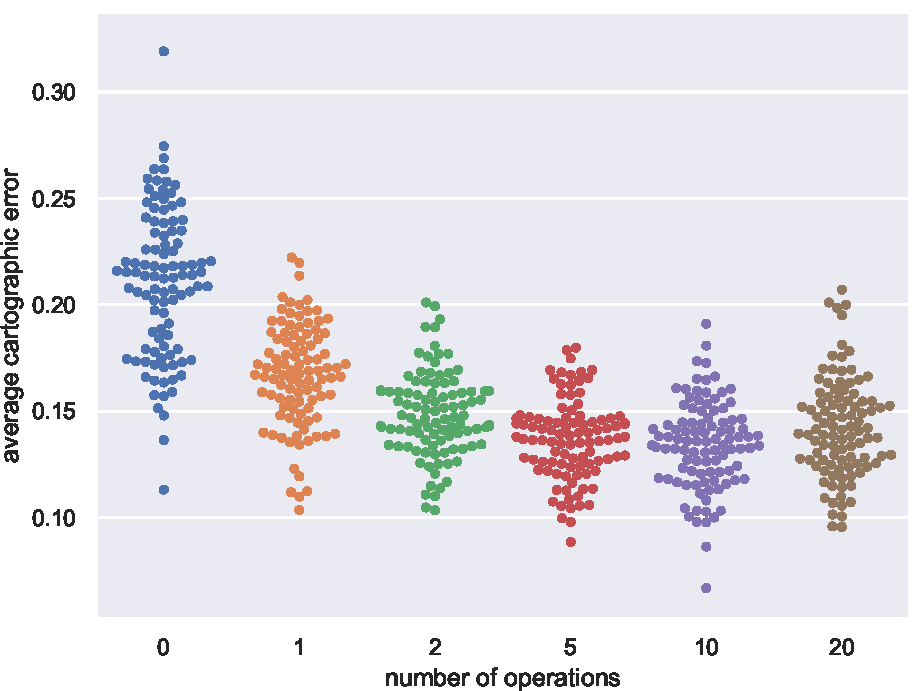
\includegraphics[width=0.47\textwidth]{Resources/Evaluation-AverageCartographicError-t.pdf}}
	\quad
	\subfigure{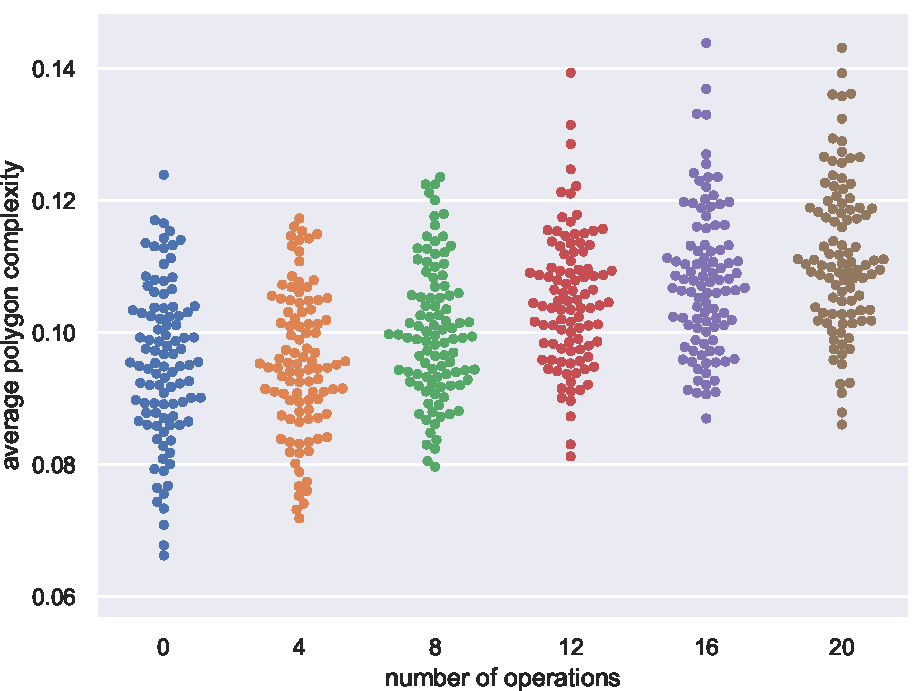
\includegraphics[width=0.47\textwidth]{Resources/Evaluation-AveragePolygonComplexity-t.pdf}}
	\subfigure{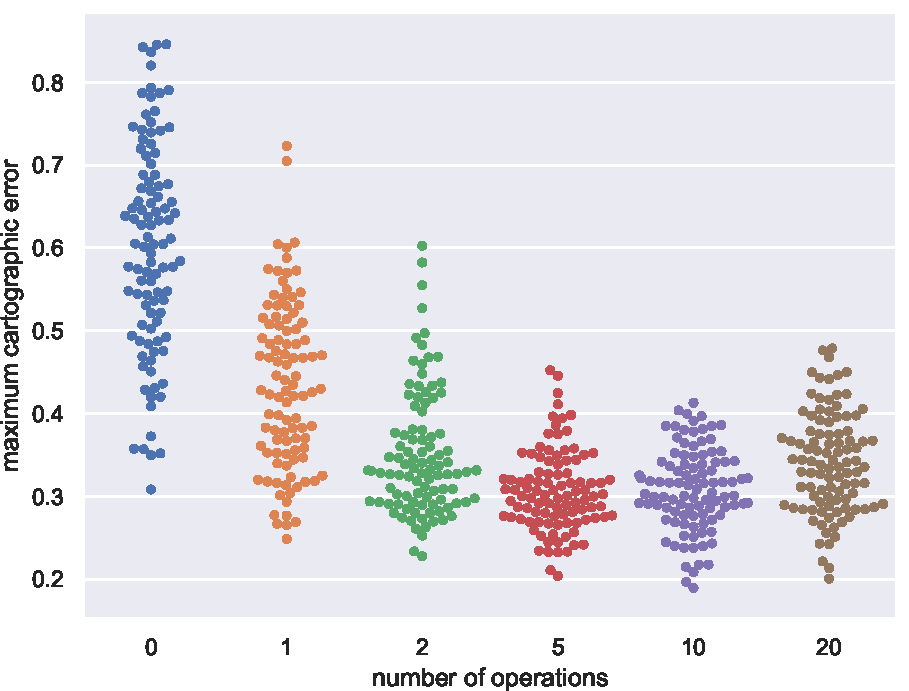
\includegraphics[width=0.47\textwidth]{Resources/Evaluation-MaximumCartographicError-t.pdf}}
	\quad
	\subfigure{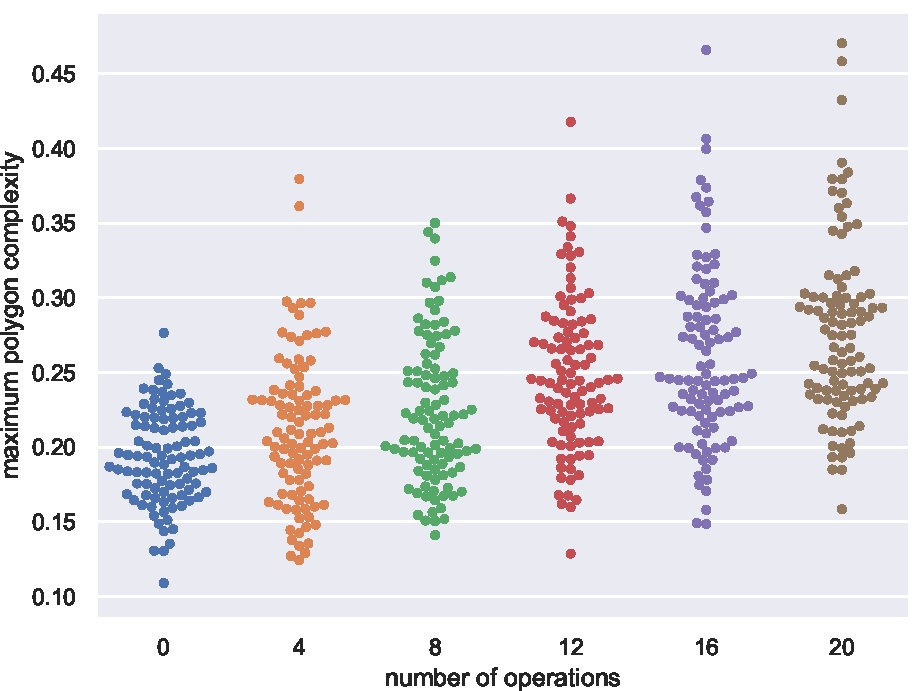
\includegraphics[width=0.47\textwidth]{Resources/Evaluation-MaximumPolygonComplexity-t.pdf}}
	\caption{Quality metrics of 100 randomized instances after applying a different number of operations $t$, with $n = 20$, $\alpha = 0$, and $\beta = 0$.}
	\label{fig:experimental-evaluation-variable-number-of-operations}
\end{figure}

We can see that as we apply more operations, the cartographic error decreases; and very quickly so, with cartographic errors after $t = 5$ operations being almost indistinguishable.
We believe that this is because for larger values of $t$, the force-directed optimization algorithm is given more time overall to optimize the statistical accuracy of the maps, amongst other features.

The polygon complexity, on the other hand, increases over time.
When processing topology-altering operations, additional subdivision vertices may be are inserted to prevent the introduction of edge crossings, potentially creating shapes that aren't locally fat in the process.
The optimization algorithm obviously tries to improve the local fatness of the involved regions afterwards, but appears unable to do so until around $t = 16$, where it seems to become able to counteract these effects and to prevent further degradation.
In \cref{sect:future-work} we discuss an approach to verify whether this change indeed happens over time, or lies in the nature of the arrangement of the regions in the different test instances.

The maximum cartographic error and polygon complexity over all regions of the map paint a picture with similar trends but greater mean and variance as outliers have a greater impact of the overall map quality.

\vspace{1cm}

The effect of the initial number of clusters $n$ on the maps' quality is shown in \cref{fig:experimental-evaluation-variable-number-of-vertices}.

\begin{figure}[H]
	\centering
	\subfigure{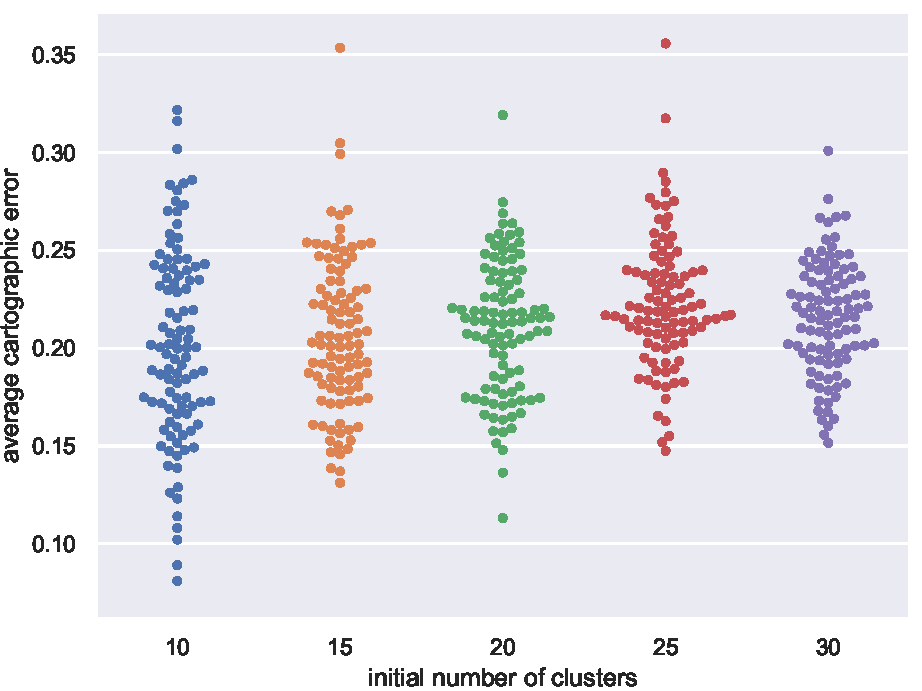
\includegraphics[width=0.47\textwidth]{Resources/Evaluation-AverageCartographicError-n.pdf}}
	\quad
	\subfigure{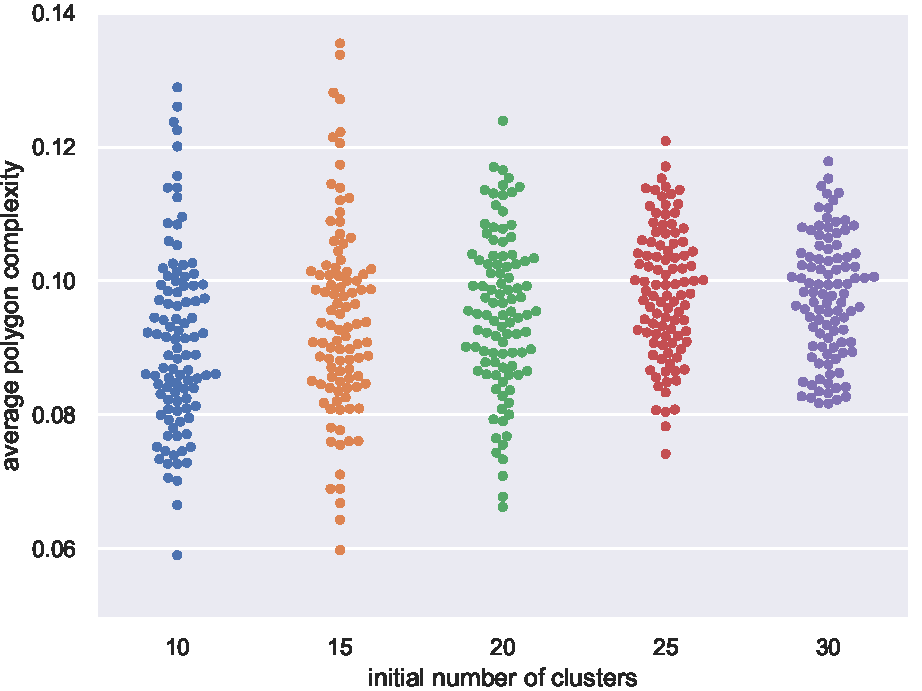
\includegraphics[width=0.47\textwidth]{Resources/Evaluation-AveragePolygonComplexity-n.pdf}}
	\subfigure{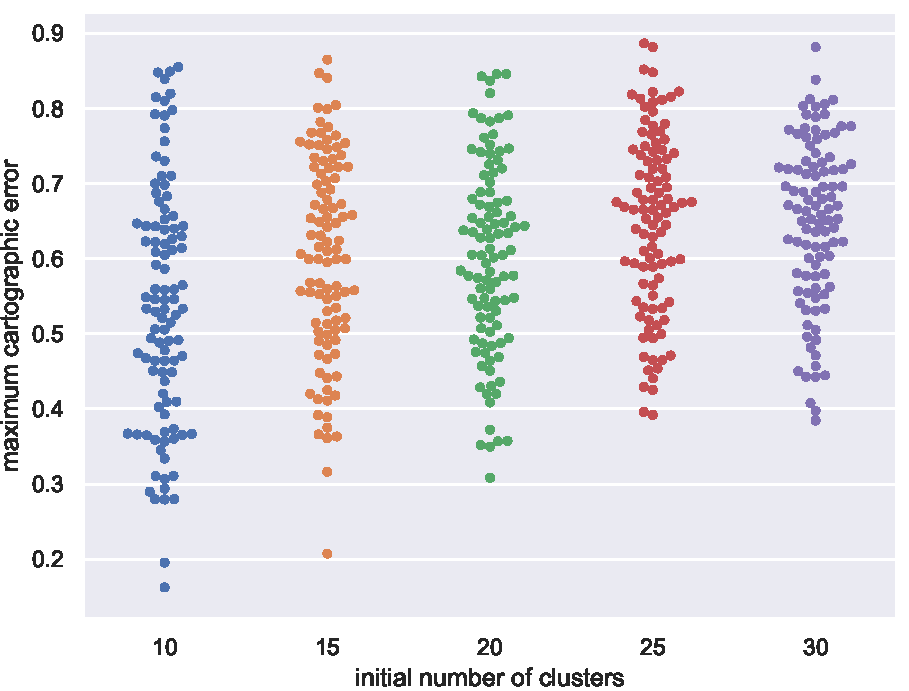
\includegraphics[width=0.47\textwidth]{Resources/Evaluation-MaximumCartographicError-n.pdf}}
	\quad
	\subfigure{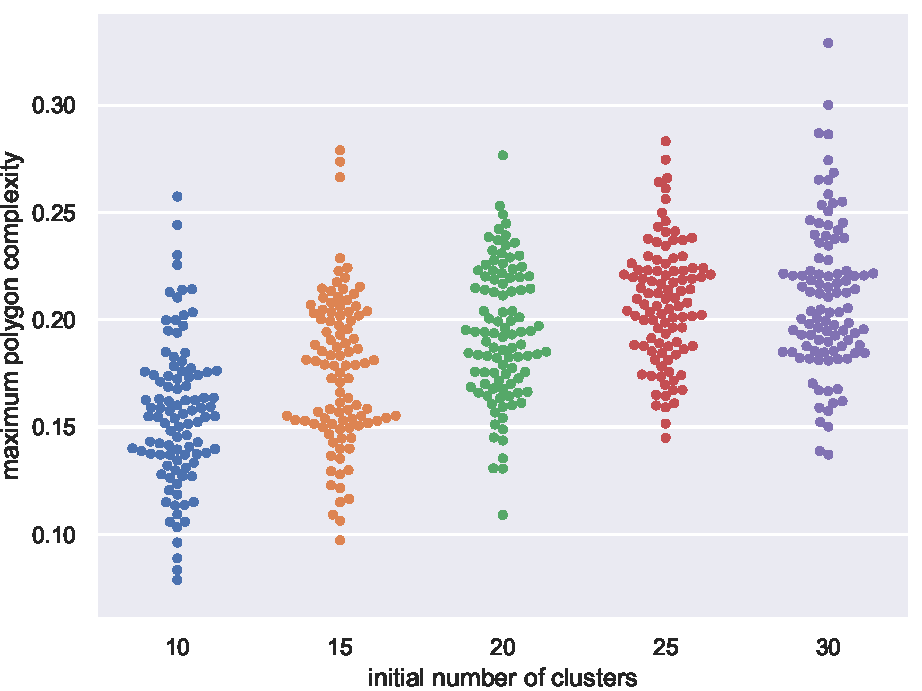
\includegraphics[width=0.47\textwidth]{Resources/Evaluation-MaximumPolygonComplexity-n.pdf}}
	\caption{Quality metrics of 100 randomized instances with different numbers of clusters $n$, with $\alpha = 0$, $\beta = 0$, and $t = 0$.}
	\label{fig:experimental-evaluation-variable-number-of-vertices}
\end{figure}

The average cartographic error across all instances appears largely unaffected by input size.
Its variance decreases though as we increase the number of clusters.
This makes sense, because as there are more clusters, the impact an outlier has on the average cartographic error decreases.

Regarding the polygon complexity, a slight increase in complexity for larger input sizes can be seen in the plot.
We believe that this is because for larger instances, there is simply more room for challenging constructs that require higher polygon complexity to visualize correctly.

With a larger number of clusters, there come more potential outliers that can negatively affect the instances' maximum cartographic errors and polygon complexities.
We therefore see more pronounced trends for these two metrics.

\clearpage

\Cref{fig:experimental-evaluation-variable-nesting-ratio-and-bias} shows the effects of different combinations of nesting ratio $\alpha$ and nesting bias $\beta$ on the maps' quality.

\begin{figure}[H]
	\centering
	\subfigure{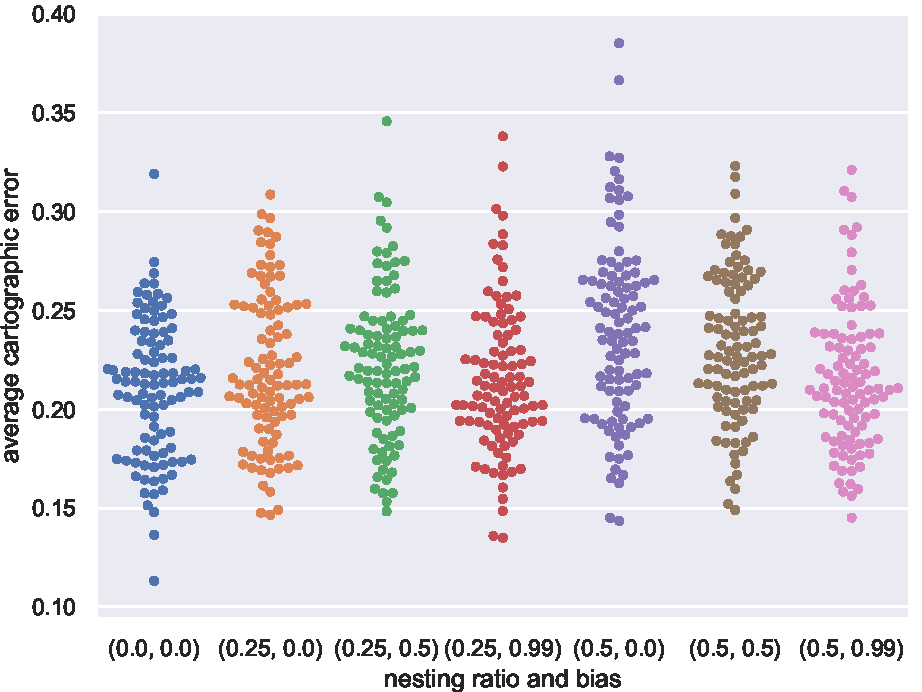
\includegraphics[width=0.47\textwidth]{Resources/Evaluation-AverageCartographicError-ab.pdf}}
	\quad
	\subfigure{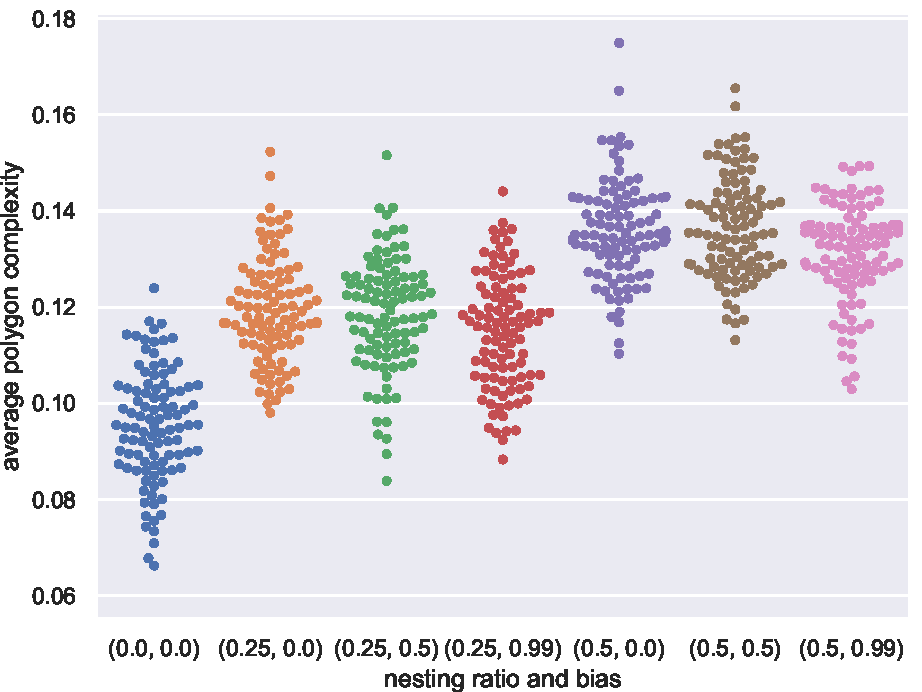
\includegraphics[width=0.47\textwidth]{Resources/Evaluation-AveragePolygonComplexity-ab.pdf}}
	\subfigure{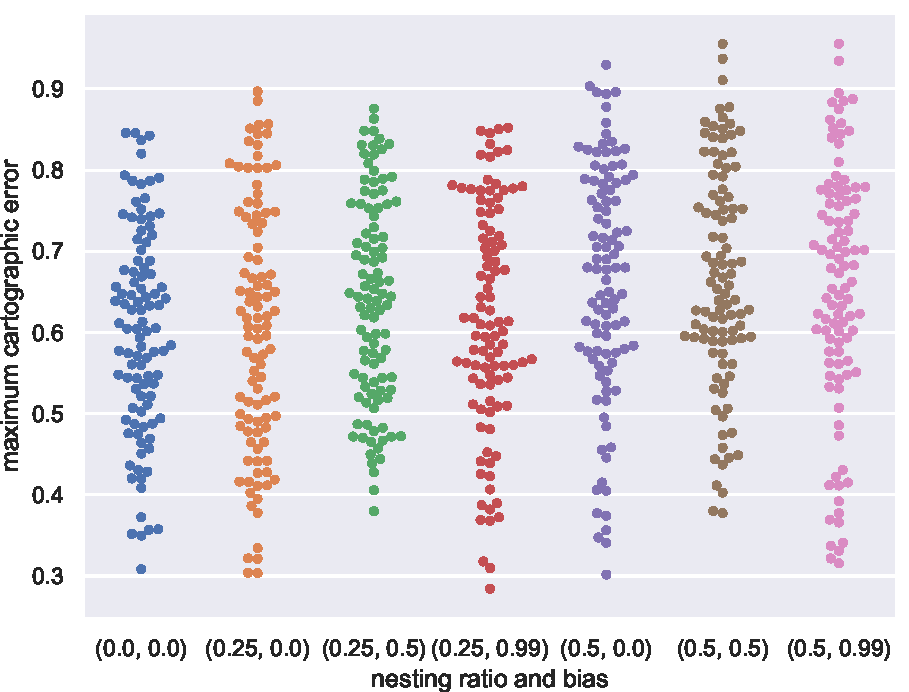
\includegraphics[width=0.47\textwidth]{Resources/Evaluation-MaximumCartographicError-ab.pdf}}
	\quad
	\subfigure{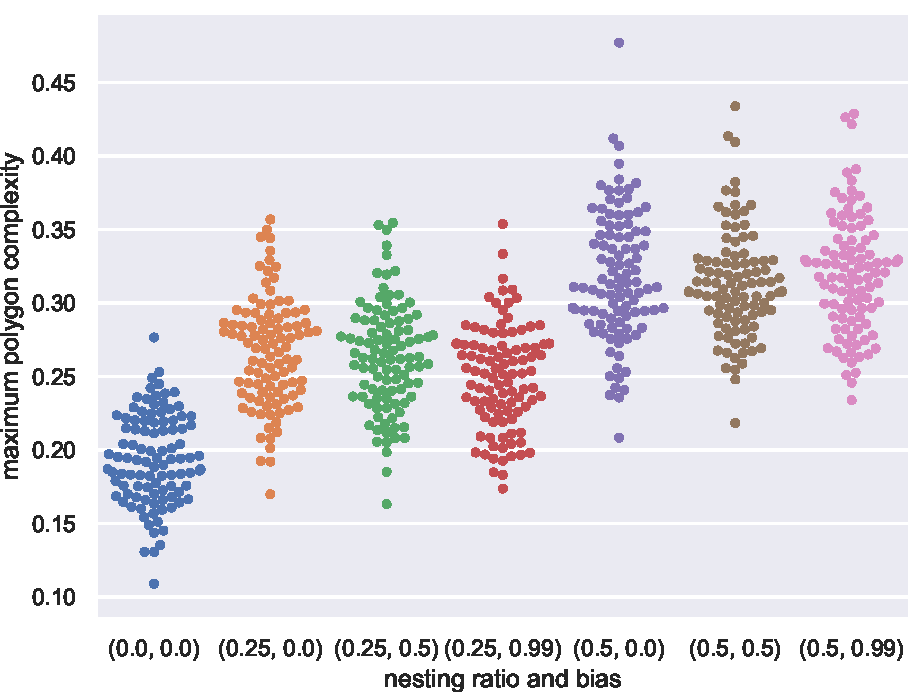
\includegraphics[width=0.47\textwidth]{Resources/Evaluation-MaximumPolygonComplexity-ab.pdf}}
	\caption{Quality metrics of 100 randomized instances with different nesting ratios $\alpha$ and nesting biases $\beta$, with $n = 20$ and $t = 0$.}
	\label{fig:experimental-evaluation-variable-nesting-ratio-and-bias}
\end{figure}

We cannot see any effect of statistical significance of nesting ratio and bias on the maps' cartographic error.

For the polygon complexity, however, the nesting ratio $\alpha$ has a pronounced impact.
The figure clearly shows that instances with $\alpha = 0.25$ tend to have higher polygon complexities than instances with $\alpha = 0$, and instances with $\alpha = 0.5$ even higher ones, regardless of nesting bias $\beta$.
A possible explanation is that by nesting vertices of the cluster graph into existing triangles, we create internal vertices with low degree.
The regions of the map corresponding to these vertices are therefore surrounded by few neighboring regions which are inevitably more complex as these few regions have to span the entire boundary of the original region.

It also appears as if for fixed nesting ratio $\alpha$, the nesting bias $\beta$ slightly reduces the map's polygon complexity.
This observation isn't significant enough to jump to any conclusions though.

Again, the maximum polygon complexity over all regions of the map exhibits the same overall trend but with a larger spread.




\clearpage
\todo{Pictures of maps generated by our framework!}

%maybe also a before/after as in short sequence of operations?
%different number of countries?

\clearpage
\section{Exemplary Maps}
\label{sect:exemplary-maps}

In this section, we showcase a range of maps produced by our framework.
\Cref{fig:exemplary-maps-dynamics} shows how such a map evolves over time as the underlying cluster graph changes.
\Crefrange{fig:exemplary-maps-small}{fig:exemplary-maps-large} show representative maps for different numbers of regions $n \in \{10,20,30\}$.

\newcommand{\bigdrawing}[1]{\setlength\fboxsep{0pt}\colorbox{gray!10}{\makebox(190,190){\includegraphics[width=190pt,height=190pt,keepaspectratio]{#1}}}}
\newcommand{\smalldrawing}[1]{\setlength\fboxsep{0pt}\colorbox{gray!10}{\makebox(120,111){\includegraphics[width=120pt,height=111pt,keepaspectratio]{#1}}}}

\begin{figure}[H]
\centering
\begin{tabular}{lc}
\begin{minipage}{0.62\textwidth}
\subfigure[]{\smalldrawing{Resources/Evaluation-Example-Dynamics-AE097F3A-14FD-4735-A19B-8FD343CA3346-0.pdf}\quad\smalldrawing{Resources/Evaluation-Example-Dynamics-AE097F3A-14FD-4735-A19B-8FD343CA3346-0-P.pdf}}
\subfigure[]{\smalldrawing{Resources/Evaluation-Example-Dynamics-AE097F3A-14FD-4735-A19B-8FD343CA3346-1.pdf}\quad\smalldrawing{Resources/Evaluation-Example-Dynamics-AE097F3A-14FD-4735-A19B-8FD343CA3346-1-P.pdf}}
\subfigure[]{\smalldrawing{Resources/Evaluation-Example-Dynamics-AE097F3A-14FD-4735-A19B-8FD343CA3346-2.pdf}\quad\smalldrawing{Resources/Evaluation-Example-Dynamics-AE097F3A-14FD-4735-A19B-8FD343CA3346-2-P.pdf}}
\subfigure[]{\smalldrawing{Resources/Evaluation-Example-Dynamics-AE097F3A-14FD-4735-A19B-8FD343CA3346-3.pdf}\quad\smalldrawing{Resources/Evaluation-Example-Dynamics-AE097F3A-14FD-4735-A19B-8FD343CA3346-3-P.pdf}}
\end{minipage}&
\raisebox{-0.45\height}{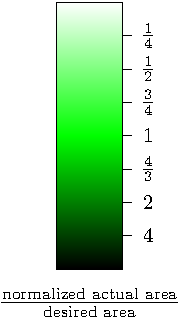
\includegraphics{Resources/Evaluation-Example-Dynamics-Legend.pdf}}
\end{tabular}
	\caption{Exemplary evolution of the generated map for an input graph with $n = 10$ at different points in time $t \in \{0,1,2,3\}$. The lightness of the region colors in the right column represents the pressure in the respective regions, with lighter regions having lower pressure than darker regions. From (a) to (b) the green-purple boundary is flipped, from (b) to (c) the red-blue boundary is flipped, and eventually from (c) to (d) the blue region is removed.}
	\label{fig:exemplary-maps-dynamics}
\end{figure}

\clearpage

\begin{figure}[H]
	\centering
	\bigdrawing{Resources/Evaluation-Example-n10-0F69CDD9-EAAD-4F81-934F-8BA98B1424F6-2.pdf}
	\bigdrawing{Resources/Evaluation-Example-n10-9A841901-DFA0-4ECD-A758-87E1C8A1D0D0-0.pdf}
	\caption{Exemplary maps produced by our framework for $n = 10$.}
	\label{fig:exemplary-maps-small}
\end{figure}

\begin{figure}[H]
	\centering
	\bigdrawing{Resources/Evaluation-Example-n20-450053F2-5F0A-4CFE-8A08-92CC201A07B9-0.pdf}
	\bigdrawing{Resources/Evaluation-Example-n20-AE097F3A-14FD-4735-A19B-8FD343CA3346-0.pdf}
	\caption{Exemplary maps produced by our framework for $n = 20$.}
	\label{fig:exemplary-maps-medium}
\end{figure}

\begin{figure}[H]
	\centering
	\bigdrawing{Resources/Evaluation-Example-n30-9BA67779-50C2-483B-8E81-916125D5D3F7-0.pdf}
	\bigdrawing{Resources/Evaluation-Example-n30-45D8EAD2-210C-4F04-8C7F-EA3E65484875-0.pdf}
	\caption{Exemplary maps produced by our framework for $n = 30$.}
	\label{fig:exemplary-maps-large}
\end{figure}

